\chapter{Revisão Bibliográfica}\label{cap:estArte}

Nessa revisão deve-se conter:

\begin{itemize}
    \item fazer referências a trabalhos publicados a respeito, situando a evolução do assunto;
    \item apenas mencionar as contribuições mais importantes diretamente ligadas ao assunto;
    \item servem como base para o desenvolvimento.
\end{itemize}

\section{Como citar no Latex}

As citações podem ser diretas, quando ocorre a transcrição textual de parte da obra do autor consultado, ou indiretas, quando o texto tem base na obra do autor consultado, ou seja, o autor do trabalho cria uma paráfrase sobre as ideias dos autores consultados, com suas palavras. A paráfrase deve ser o modo principal de produção de texto na revisão da literatura.

As citações devem ser feitas de acordo com a norma e devem seguir o modelo Autor-data, em que a data é o ano. Se a citação estiver dentro de parênteses, ela deve ser destacada no texto e escrita com letras MAIÚSCULAS, se estiver fora de parênteses, deve ser escrita em letras minúsculas como segue:

\begin{itemize}
    \item único autor: Silva (2008) ou (SILVA, 2008);
    \item dois ou três autores: Tortora, Funke e Case (2000) ou  (TORTORA, FUNKE e CASE, 2000);
    \item mais de três autores: Kearney et al . (2009) ou (KEARNEY et al., 2009);
    \item No caso de haver mais de uma obra citada para o mesmo parágrafo, os autores devem aparecer em ordem ALFABÉTICA na citação, por exemplo, (CUNHA, 2009; KIRK et al., 2013; POTTER e BIRMANN , 1999; WEISS et al., 2011)
\end{itemize}

Exemplos:

De acordo com \citeonline{lu2017industry}

bla bla bla bla bla bla bla \cite{lu2017industry}

De acordo com \citeonline{sacomano2018industria}

bla bla bla bla bla bla bla \cite{sacomano2018industria}


Se a citação for textual, deve-se adicionar o número da página, como no exemplo: Segundo a NBR 10520 (2002, p. 2), "As citações diretas, no texto, de até três linhas, devem estar contidas entre aspas duplas. As aspas simples são utilizadas para indicar citação no interior de citação."

Para indicar a página utiliza-se: 

De acordo com \citeonline [p.~12] {lu2017industry} "As citações diretas, no texto, de até três linhas, devem estar contidas entre aspas duplas. As aspas simples são utilizadas para indicar citação no interior de citação."

\section{Figuras no Latex}

Ilustração é o termo genérico que abrange todo o elemento gráfico de apoio ao texto (ABNT NBR 14724, 2011). Na área técnica o termo mais comum é: \textbf{Figura}

Digamos que haja um texto e que ele seja ilustrado por uma figura. Cuidar com a expressão abaixo e acima. Usar a expressão “a seguir”, pois a figura sempre estará “a seguir” e, muitas vezes a figura “abaixo” acaba ficando “acima” na próxima página, por causa da inserção de mais texto no documento.

A forma de apresentação das ilustrações é definida pela NBR 14724 (2011) e tem a estrutura apresentada a seguir.

\begin{itemize}
    \item Título deve ficar ACIMA da figura (colocar o ponteiro do mouse sobre a figura e clicar no botão direito que aparece o comando Legenda). O título não leva ponto ao seu final;
    \item Figura propriamente dita – propriedades, dimensionamento, posicionamento (colocar o ponteiro do mouse sobre a figura e clicar no botão direito que aparecem os comandos Tamanho e posição e Formatar imagem);
    \item Fonte – logo após a figura.
\end{itemize}

\begin{figure}[h]
    \centering
    \caption{Perspectiva da superfície de Marte}
    \centering
    
\includegraphics[width=.40\linewidth]{images/latex_00.jpg}
    \caption*{Fonte: \cite{lu2017industry} }
    \label{fig:my_label}
\end{figure}

É importante esclarecer que TODOS os elementos de apoio ao texto — Figuras, Tabelas, Referências, Apêndices e Anexos — além das equações (que são elementos de texto destacados) devem ser citados no texto, ou seja, nada é inserido no trabalho sem que o texto lhe faça a devida referência. Exemplo: na Figura \ref{fig:my_label}.... Figura \ref{fig:my_label2}

\begin{figure}[h]
    \centering
    \caption{Perspectiva da superfície de Marte}
    \centering
    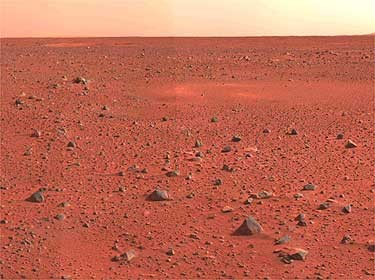
\includegraphics[width=.65\linewidth]{images/marte.jpg}
    \caption*{Fonte: Northeastern News \footnotemark , 2020}
    \label{fig:my_label2}
\end{figure}

\begin{figure}[h]
    \centering
    \caption{Perspectiva da superfície de Marte}
    \centering
    
\includegraphics[width=.40\linewidth]{images/latex_00.jpg}
    \caption*{Fonte: \cite{lu2017industry} }
    \label{fig:my_label4}
\end{figure}

\begin{figure}[h]
    \centering
    \caption{Perspectiva da superfície de Marte}
    \centering
    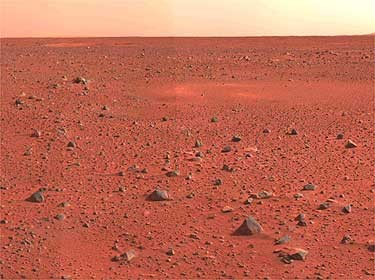
\includegraphics[width=.65\linewidth]{images/marte.jpg}
    \caption*{Fonte: Northeastern News \footnotemark , 2020}
    \label{fig:my_label3}
\end{figure}

Na Figura \ref{fig:my_label2}  e na Figura \ref{fig:my_label3} se apresenta uma sugestão para a indicação da fonte de figuras obtidas da internet. Em vez de se colocar o endereço completo (string) do qual se copiou a imagem após a palavra fonte, ele pode ser deslocado para uma nota de rodapé e, no seu lugar, se coloca a indicação do sítio no qual se encontrava a imagem. Dessa forma, o endereço da internet fica associado ao sítio pelo número da nota de rodapé, favorecendo a estética. 

\footnotetext{https://news.northeastern.edu/2019/07/17/northeastern-university-looks-back-at-the-moon-landing-50-years-later-mars-and-beyond/. Acesso em 28/05/2020}

\section{Equações no Latex}

Na Equação \ref{eq:eq1} é apresentado um exemplo de equação com apenas uma linha.

\begin{equation}
\label{eq:eq1}
        \partial \Dot{S} = \left( \frac{\partial \Dot{S} } {\partial S} \right)_0 \cdot \partial S 
\end{equation}

Na Equação \ref{eq:eq2} é apresentado um exemplo de equação com múltiplas linhas.

\begin{equation}
\label{eq:eq2}
    \begin{split}
        \partial \Dot{S} = \left( \frac{\partial \Dot{S} } {\partial S} \right)_0 \cdot \partial S \\
                         = \left( \frac{\partial \Dot{I} } {\partial S} \right)_0 \cdot \partial S \\
                         = \left( \frac{\partial \Dot{R} } {\partial I} \right)_0 \cdot \partial I
    \end{split}
\end{equation}

Na Equação \ref{eq:eq3} é apresentado um exemplo de um sistema equações com múltiplas linhas.
\begin{equation}
\label{eq:eq3}
    \begin{split}
        \begin{cases}
            \partial \Dot{S} =  \left( \frac{\partial \Dot{S} } {\partial S} \right)_0 \cdot \partial S \\
            \partial \Dot{I} = \left( \frac{\partial \Dot{I} } {\partial S} \right)_0 \cdot \partial S \\
            \partial \Dot{R} = \left( \frac{\partial \Dot{R} } {\partial I} \right)_0 \cdot \partial I
        \end{cases}
    \end{split}
\end{equation}


